% This template is designed to be used with the `article' class, and was developed using MikTex 2.9.
\documentclass[12pt,letter]{article}

% poma_style.sty is used to generate the appropriate format
\usepackage{poma_style}

% Include any other packages and definitions needed
\usepackage{graphicx}
\usepackage{amsmath,amsfonts,bm}
\usepackage{courier}

\newcommand{\eps}{\varepsilon}

\begin{document}

\section{POMA Overview}

\textsl{Proceedings of Meetings on Acoustics} (POMA) is an editor-reviewed, open-access, online journal published by the Acoustical Society of America (ASA). Articles originate as papers presented at semiannual ASA meetings or at other cosponsored meetings. Both researchers and practitioners are encouraged to submit manuscripts to POMA. 

Because of rapid editorial processing, the Proceedings offers a timely venue for viewing the most current work in the broad field of acoustics. All manuscripts are reviewed from the standpoints of clarity and correctness by an Associate Editor and are published online shortly after being accepted.  

Articles are published within volumes tied to Society meetings and typically organized by primary topical area: Acoustical Oceanography, Animal Bioacoustics, Architectural Acoustics, Biomedical Acoustics, Education in Acoustics, Engineering Acoustics, Musical Acoustics, Noise, Physical Acoustics, Psychological and Physiological Acoustics, Signal Processing in Acoustics, Speech Communication, Structural Acoustics and Vibration, and Underwater Acoustics.


\section{POMA Policies}

\subsection{Eligible Submissions}

Papers from any prior ASA meeting or from designated cosponsored conferences are eligible for submission to POMA. Coauthor approval must be obtained prior to submission. Verification that the author list is complete and of coauthor approval occurs as part of the editorial process.

\subsection{Acceptance Criteria}

In principle, any ASA meeting paper, including case studies and preliminary or limited-scope investigations, is suitable for POMA. The criteria of clarity and correctness are intended to ensure manuscripts reflect the high-quality work presented at ASA meetings. Authors are expected to:
\begin{itemize}
	\item Present their work in clear, grammatically correct English
	\item Lay out the camera-ready manuscript in a professional manner
	\item Ensure all figures are readable and attractive
	\item Provide adequate reference to prior literature used in the work
	\item Strive for technical correctness. While the level of review does not approach that of JASA, POMA does not intend to publish any paper where the initial premises, reported results, or conclusions are wrong. 
\end{itemize}

Reasons for ultimately rejecting a POMA manuscript include prior publication or copyright violations, promotion of commercial products, technical unreasonableness, or failure to make changes as indicated by the associate editor or manuscript manager. 

\subsection{Copyright}

Although POMA is open-access, articles published in POMA are copyrighted by the ASA unless authored by a U.S. or Canadian government employee as part of his/her official duties. The ASA copyright agreement form explains how POMA authors retain extensive rights as to subsequent use of articles, including allowing republication and reposting.

If authors wish to use copyrighted material in an article, it is their responsibility to obtain permission from the copyright holder.

\subsection{Prior Publication}

Publication in POMA does not constitute prior publication by the Acoustical Society of America's fully-reviewed journals, The Journal of the Acoustical Society of America and its Express Letters section.


\section{Manuscript Preparation and Submission}

To help authors prepare the article cover page and manuscript files, the checklist used by the POMA manuscript manager in the initial quality review is located at http://scitation.aip.org/POMA under the Authors tab.

\subsection{Cover Page Preparation}

As part of the manuscript preparation, authors create a pdf cover page using the MS Word or \LaTeX~templates provided under the Authors tab on Scitation. This is submitted as a separate document. Three items to note:

\begin{itemize}
	\item The author name, affiliation, and email address must match the conference-submitted metadata. Failure to do so without explanation in the submission comments will trigger a failed quality check and delay processing.  Note that changes in author order or additions are acceptable, but any deletions must be accompanied with an explanation.
	\item The abstract need not be identical to the conference-submitted form.  Rather, the abstract should be updated to contain results and principal conclusions.
	\item Acknowledgments should be included at the end of the manuscript, not enclosed in brackets in the abstract (as is done in ASA meeting abstracts).
\end{itemize}

\subsection{Manuscript Format}

All manuscripts submitted to POMA must be camera-ready pdf files corresponding to a talk or poster. The paper should look like a proceedings paper from a mainstream technical society. This \LaTeX~document with the associated style document \texttt{poma\_style.sty} may be used as a template.  Alternatively, authors may visit the POMA website to view recent papers for suitable formats, but should recognize that not every previously published article is still considered acceptable.  \textbf{Papers that represent a collection of slides with little or no accompanying text will ordinarily require significant revision.}

\subsubsection{Guidlines}

The following manuscript guidelines apply:

\begin{itemize}
	\item File begins with the introduction (cover page already contains author information)
	\item $8.5\times 11$ inch page in portrait orientation
	\item No page numbers and no headers/footers of any sort. These are added during publication
	\item 14 pages maximum for the manuscript file (15 pages total, including cover page)
	\item 1-inch side margins and at least 0.75-inch top/bottom margins
	\item Font should be 10-12 pt and single-spaced. Times New Roman is used to generate the cover page and manuscript header and footers, but other fonts (e.g., Arial, Calibri, Cambria, Courier) are allowed.
	\item Figures or tables must be embedded in the pdf file consistent with a camera-ready document, rather than grouped at the end
	\item Color figures are encouraged
	\item No active links in the manuscript. Multimedia may be included via a reference to an external link, with the author assuming responsibility for ensuring that the files be readily accessible
	\item If slides from the talk are to be used directly as figures:
\begin{itemize}
	\item Adjust figure resolution to minimize file size while maintaining sufficient quality
	\item No more than two slides per page
	\item All header and footer information unnecessary for conveying scientific content should be removed, including logos and slide numbers
	\item Each slide should have a figure number and caption, and that figure should be referenced explicitly in the text, as is customary for a written paper.
\end{itemize}
\end{itemize}
Including the package \texttt{poma\_style.sty} will incorporate most of these guidelines automatically.

\subsubsection{Including references, figures, tables, and equations}

A POMA manuscript will normally have references and some combination of figures, tables, and equations. In this template document, there are included text styles for both captions and references.  Figure and table captions should be centered if they are only one line and be full justified if they are longer than one line.  Additional instructions regarding inclusion and automated numbering of, and cross-referencing to, these different elements are given below.

A separate References section should be at the end of the document and labeled References or Bibliography. This allows Google Scholar and other indexing services to locate them.  No specific formatting is required, but either of the two JASA formats is preferred. References may be inserted as endnotes just below the ``Reference'' heading, allowing for easy cross-referencing throughout the document or inserted manually. An example endnote is included here.\cite{daigle79}  While in this template the bibliography is fully incorporated into the \texttt{.tex} file, any method of generating the bibliography is acceptable.

When referencing to figures, the abbreviation ``Fig.'' followed by the figure number should be used, except when the reference comes first in a sentence, where ``Figure'' should replace ``Fig.''  Two example sentences referencing a figure are: Figure~\ref{fig:gem60} shows a distant view of GEM-60 solid rocket motor firing along with some geometry.  As can be seen in the pictures in Fig.~\ref{fig:gem60}, snow covered the ground during the experiment.

\begin{figure}
	\centering
	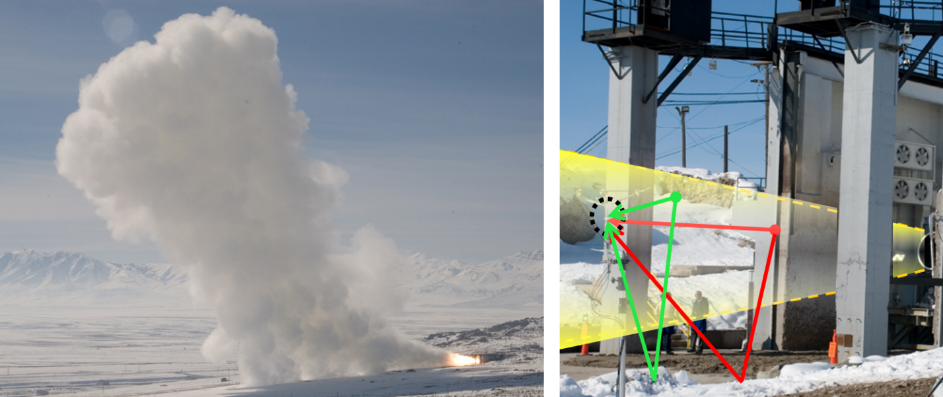
\includegraphics{GEM60_Picture}
	\caption{\label{fig:gem60}Distant view of a GEM-60 solid rocket motor firing.}
\end{figure}

References to tables are never abbreviated.  As an example, rocket specifications for the rocket motor in Fig.~\ref{fig:gem60} are provided below in Table~\ref{tab:rocket}.

\begin{table}
	\centering
	\caption{\label{tab:rocket}Sample rocket parameters.}
\begin{tabular}{lcl}
	\textbf{Parameter} & \textbf{Symbol} & \textbf{Value} \\ \hline
	Thrust & $T$ & 870 kN \\
	Diameter & $D$ & 1.2 m \\
	Centerline velocity & $v_j$ & 2000 m/s
\end{tabular}
\end{table}

Equations should ordinarily be numbered, which is performed automatically by \LaTeX.  The following sentence illustrates cross referencing to a figure and an equation: The noise from the rocket plume in Fig. 1 can be modeled using the cylindrical wave functions in Eq. (1).

\begin{equation}
	\Phi_{l,k_z}(r,\phi,z) \equiv \frac{H_l^{(1)}(k_rr)}{H_l^{(1)}(k_rr_0)} e^{il\phi}e^{ik_zz}, \hspace{10mm} r\ge r_0.
\end{equation}




\section{Submission}

Manuscripts are submitted via http://www.editorialmanager.com/poma/ as a camera-ready pdf document. Users new to Editorial Manager must first register for a unique author identification number at http://orcid.org and then create an Editorial Manager user account.


\section{Editorial Process Overview}

\begin{enumerate}
	\item The author prepares the pdf cover page and manuscript as separate pdf documents.
\begin{enumerate}
	\item \textbf{Do not upload Word or .tex files to Editorial Manager.}
	\item \textbf{Cover page information (affiliations, etc.) must match author metadata.}
	\item \textbf{It is imperative that page size and margin requirements are followed.}
\end{enumerate}
	\item If applicable, coauthor approval should be obtained prior to submission. Coauthors will be required to confirm their approval during the editorial process. 
	\item The corresponding author logs onto POMA Editorial Manager, fills out the required submission information, and uploads the cover page and manuscript in pdf format.
	\item The POMA Manuscript Manager performs an initial quality check of the manuscript, in accordance with the checklist.
	\item Once the article passes the initial quality review, the assigned Associate Editor reviews the manuscript for clarity and correctness. In unusual cases or for some cosponsored meetings, external reviewers may be consulted.
	\item The corresponding author receives an email indicating acceptance, rejection, or required revisions.
	\item After acceptance, headers and footers are added to the manuscript and the accepted article appears within the appropriate POMA volume.  \textbf{The acceptance letter will invite the author to submit a marked-up pdf document with any requested minor typographical changes. This must occur within 24 hrs; once the publication process has begun, no changes will be considered.}
\end{enumerate}


\section{Conclusion}

A conclusion or concluding discussion should be included.


\section*{Acknowledgments}

Acknowledgments, if any, follow the conclusion section.

\appendix

\section*{Appendix A}

Appendices, if necessary, can go here. However, given the scope of a typical POMA article, the use of an appendix would be uncommon.


\begin{thebibliography}{9}

\bibitem{daigle79}
	G. A. Daigle, ``Effects of atmospheric turbulence on the interference of sound waves above a finite impedance boundary'', \textsl{J. Acoust. Soc. Am.} \textbf{65}, 45-49 (1979).

\end{thebibliography}



\end{document}










































